\documentclass[tikz,border=6pt]{standalone}
\usepackage[T1]{fontenc}
\usepackage[utf8]{inputenc}
\usepackage{amsmath,amssymb}
\usepackage{tikz}
\usetikzlibrary{automata,positioning,arrows.meta,shapes.geometric,calc,fit}
\tikzset{
    >=Stealth,
    every state/.style={minimum size=8mm, inner sep=1pt, font=\small},
    flow/.style={rectangle, rounded corners, draw, align=center, minimum width=3.1cm, minimum height=0.9cm},
    decision/.style={diamond, draw, aspect=2.0, align=center, inner sep=1.5pt},
    terminal/.style={ellipse, draw, align=center, minimum width=2.4cm, minimum height=0.85cm},
    module/.style={rectangle, draw, rounded corners, align=center, minimum width=3.4cm, minimum height=1.0cm},
    data/.style={rectangle, draw, align=center, minimum width=3.2cm, minimum height=0.9cm}
}
\begin{document}
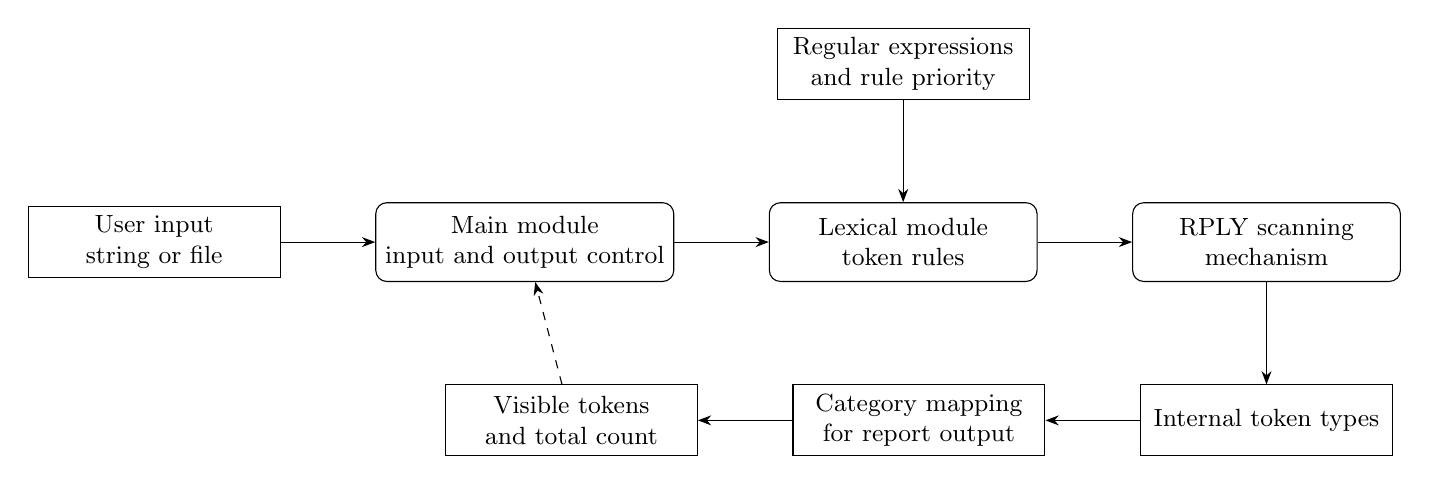
\begin{tikzpicture}[node distance=13mm and 12mm, font=\small, ->]
    \node[data] (user) {User input\\string or file};
    \node[module, right=of user] (main) {Main module\\input and output control};
    \node[module, right=of main] (lexer) {Lexical module\\token rules};
    \node[module, right=of lexer] (rply) {RPLY scanning\\mechanism};

    \node[data, above=of lexer] (rules) {Regular expressions\\and rule priority};
    \node[data, below=of rply] (internal) {Internal token types};
    \node[data, left=of internal] (mapping) {Category mapping\\for report output};
    \node[data, left=of mapping] (visible) {Visible tokens\\and total count};

    \draw (user) -- (main);
    \draw (main) -- (lexer);
    \draw (lexer) -- (rply);
    \draw (rules) -- (lexer);
    \draw (rply) -- (internal);
    \draw (internal) -- (mapping);
    \draw (mapping) -- (visible);
    \draw[dashed] (visible) -- (main);
\end{tikzpicture}
\end{document}
